%%%%%%%%%%%%%%%%%%%%%%%%%%%%%%%%%%%%%%%%%
% Short Sectioned Assignment
% LaTeX Template
% Version 1.0 (5/5/12)
%
% This template has been downloaded from:
% http://www.LaTeXTemplates.com
%
% Original author:
% Frits Wenneker (http://www.howtotex.com)
%
% License:
% CC BY-NC-SA 3.0 (http://creativecommons.org/licenses/by-nc-sa/3.0/)
%
%%%%%%%%%%%%%%%%%%%%%%%%%%%%%%%%%%%%%%%%%

%----------------------------------------------------------------------------------------
%   PACKAGES AND OTHER DOCUMENT CONFIGURATIONS
%----------------------------------------------------------------------------------------

\documentclass[paper=letter, fontsize=11pt]{scrartcl} % A4 paper and 11pt font size
\synctex=1
\usepackage[T1]{fontenc} % Use 8-bit encoding that has 256 glyphs
\usepackage{fourier} % Use the Adobe Utopia font for the document - comment this line to return to the LaTeX default
\usepackage[english]{babel} % English language/hyphenation
\usepackage{amsmath,amsfonts,amsthm} % Math packages
%\usepackage[nolists, nomarkers]{endfloat}
\usepackage{hyperref}
\usepackage{bm}
\usepackage{graphicx}
\usepackage[section]{placeins}
\usepackage{sectsty} % Allows customizing section commands
\allsectionsfont{\normalfont\scshape} % Make all sections centered, the default font and small caps

\usepackage{fancyhdr} % Custom headers and footers
\pagestyle{fancyplain} % Makes all pages in the document conform to the custom headers and footers
\fancyhead{} % No page header - if you want one, create it in the same way as the footers below
\fancyfoot[L]{} % Empty left footer
\fancyfoot[C]{} % Empty center footer
\fancyfoot[R]{\thepage} % Page numbering for right footer
\renewcommand{\headrulewidth}{0pt} % Remove header underlines
\renewcommand{\footrulewidth}{0pt} % Remove footer underlines
\setlength{\headheight}{13.6pt} % Customize the height of the header

\numberwithin{equation}{section} % Number equations within sections (i.e. 1.1, 1.2, 2.1, 2.2 instead of 1, 2, 3, 4)
\numberwithin{figure}{section} % Number figures within sections (i.e. 1.1, 1.2, 2.1, 2.2 instead of 1, 2, 3, 4)
\numberwithin{table}{section} % Number tables within sections (i.e. 1.1, 1.2, 2.1, 2.2 instead of 1, 2, 3, 4)

\setlength\parindent{0pt} % Removes all indentation from paragraphs -
                          % comment this line for an assignment with
                          % lots of text
\setlength\parskip{12pt}

%----------------------------------------------------------------------------------------
%   TITLE SECTION
%   ----------------------------------------------------------------------------------------
%----------------------------------------------------------------------------------------
%   TITLE SECTION
%----------------------------------------------------------------------------------------

\newcommand{\horrule}[1]{\rule{\linewidth}{#1}} % Create horizontal rule command with 1 argument of height

\title{ 
\normalfont \normalsize 
\textsc{Exoplanet Patchy Cloud Project} \\ [25pt] % Your university, school and/or department name(s)
\horrule{0.5pt} \\[0.4cm] % Thin top horizontal rule
\huge Note for last two weeks\\ % The assignment title
\horrule{2pt} \\[0.5cm] % Thick bottom horizontal rule
}

\author{Yifan Zhou} % Your name

\date{\normalsize\today} % Today's date or a custom date

\begin{document}

\maketitle % Print the title
\section{Ramp effect}
% \begin{quote}
%   \begin{itemize}
% \item 2 ways
% \item check the paper
%  \end{itemize}
% \end{quote}

\begin{itemize}
\item  In \textsl{Wilkins et. al. 2013}\\
    The ramp effect is neglectable when exposure level is below \textbf{30000} electrons per pixel.
\item In \textsl{Deming et. al. 2013}\\
    They expected ramp effect to be weakly detectable in their data
    when their exposure level is about \textbf{40000} electrons per pixel.
\end{itemize}

 In our data, the maximum exposure level at the secondary image is $\sim$2000 e$^-$ per pixel, which is far below 30000 e$^-$ per pixel. Therefore the ramp effect in our case should be small enough.

 \section{ PSF photometry}
 % \begin{quote}
 %   plot PSF photometry with aperture photometry
 % \end{quote}

 \subsection{PSF Generation}
Different PSFs are generated with different filter and rolling
angle. Therefore totally there were 4 PSFs generated (F125W, Angle 1;
F125W, Angle 2; F160W, Angle 1; F160W, Angle 2). Each PSF is the
combination of all secondary object images with primary star
subtracted, that were taken with same
filter and rolling angle. The images were not re-aligned with the
secondary object centroids (reason explained later).\par

 \subsection{Result}
 \begin{figure}
   \centering
   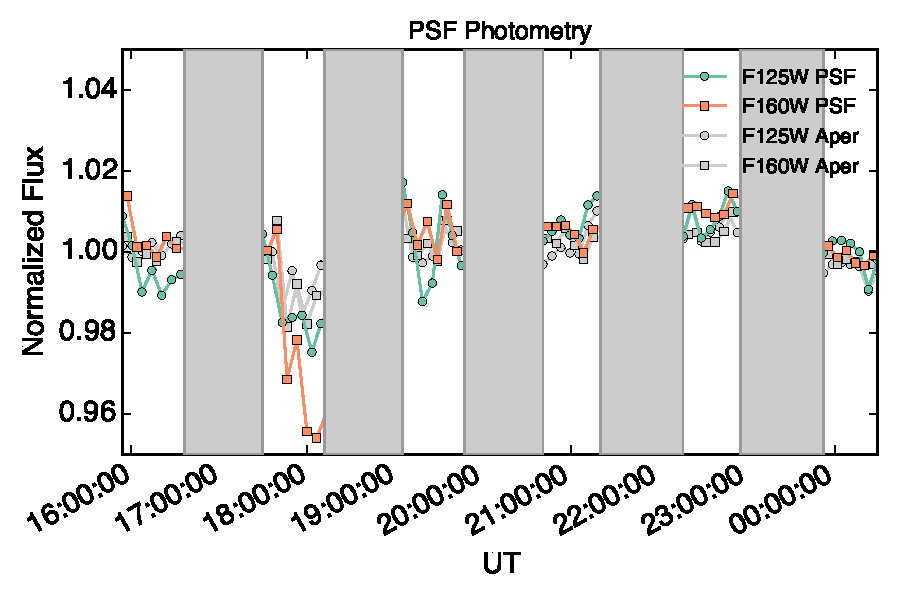
\includegraphics[width = 0.8\textwidth]{PSFPhotometry_Nov20}
   \caption{PSF fitting light curve and aperture photometry ligth
     curve}
   \label{fig:psf}
 \end{figure}

 \begin{figure}
   \centering
   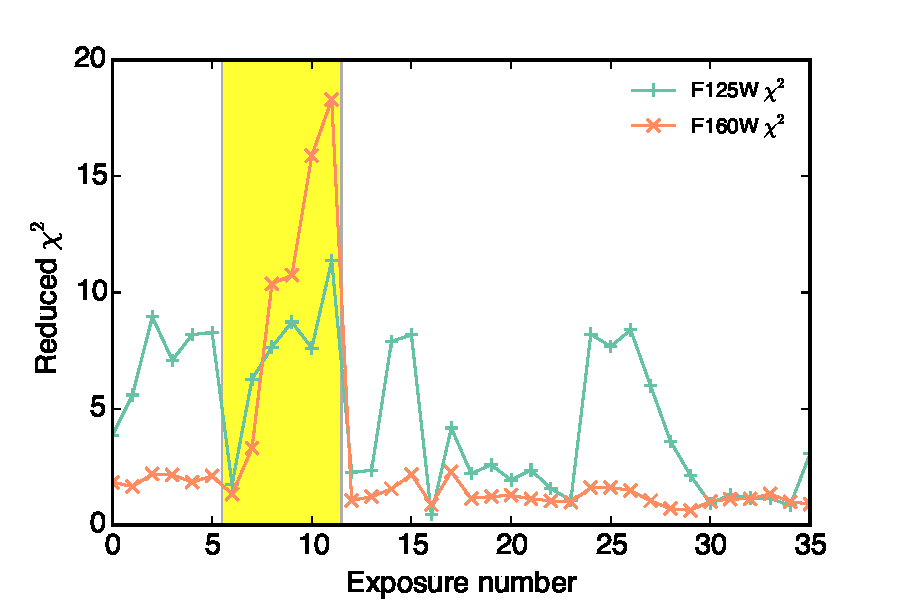
\includegraphics[width = 0.8\textwidth]{PSFFitChisq}
   \caption{PSF fitting reduced $\chi^2$. Yellow shaded patch
     indicates the 2nd orbit.}
   \label{fig:chisq}
 \end{figure}

 Preliminary PSF photometry result is presented with
 Figure \ref{fig:psf}. Colored lines are PSF photometry light curves, with
 aperture photometry light curves plotted in gray lines as
 reference. The PSF photometry results are not well correlated with
 aperture photometry especially in first two orbits. In last three
 orbits, PSF photometry seems to match better with aperture
 photometry.\par

 Figure \ref{fig:chisq} shows the reduced $\chi^{2}$ for PSF
 fitting. All F125W images fit terribly with PSF. However, most of
 F160W images have a good fit, except images taken in second
 orbit. Accordingly, the F160W PSF photometry light curve has the
 largest offset in second orbit (figure \ref{fig:psf}) comparing to
 aperture photometry.\par

\subsection{Possible Reason for Bad Fit and other problem}
% 1. for the same filter and the same rolling angle, the center of the secondary is not exactly at the same position. Using mpfit2dpeak to measure the secondary centroid, the maximum difference in both x and y direction could be as large as 0.05 pixel (measured by cross correlation). *This effect would enlarge the  fwhm of the synthesis PSF.*

% -> align the image again when generating PSF
% - fshift (a linear interpolation) will slightly change the PSF -- enlarge the FWHM, this problem will be alleviate by oversampling with a cubic interpolation, but could not be eliminated
% - without second alignment with secondary object, synthetic PSF FWHM -- 1.93 pixels
% - align again with secondary object, synthetic PSF FWHM -- 2.00 pixels.

\subsubsection{fshift changes PSF}

I checked the F160W second orbit images, and found that for the two
images that have the worst PSF fit, their secondary object images are
clearly from others' -- the FWHMs for these two images are 0.2 pixel
narrower than those for other images. However in the original images
(without registration and primary star subtraction), the PSFs for these
two images are similar to those for others.

In the mean time, I found the PSF's FWHM are enlarged by fshift, which
I guess is due to bilinear interpolation. For the original F160W
PSF, the FHWM is $\sim 1.68$ pixels. After registration and primary
subtraction, it becomes $\sim 1.9$ pixels.

I did some test and confirmed that fshift did change the PSF. I also
found over sampling the image with cubic interpolation
(\texttt{congrid(,cubic=-0.5)})first would alleviate this effect but
could not eliminate it. I guess the degree that fshift enlarge the
FHWM of PSF is related to the fractional part of the shift, but I have
not confirmed it yet.

I think fshift could make the PSF slightly unstable and could be one
of the reason for bad PSF fit. For this reason, I did not align the
image again with the centroids of secondary objects when generating
synthetic PSF because it calls
for fshift again. Actually for the cross correlation aligned images,
the maximum offset for secondary objects' positions is $\sim0.05$ pixel,
which could cause a $\sim0.1$ pixel enlargement in synthetic PSF's FWHM. On the
other hand fshift itself could enlarge the FWHM for $\sim0.1$ pixel.

\subsubsection{How to normalize the PSF? }
To get absolute flux measurement, synthetic PSF has to be
normalized. I am not sure what factor to use for the normalization.


\begin{quote}
aperture radius vs standard deviation
use aper.pro  to measure photometry and uncertainty
\end{quote}


\section{Analyze light curve}
\begin{quote}
 is the source varying
 what is the amplitude in two colors
\end{quote}

According to aperture photometry, the peak to peak variation is about
2%

\begin{quote}
  is the change periodic
\end{quote}

At least, it is difficult to find a period by eye.

\begin{quote}
  are the changes in the filter correlated
\end{quote}
As shown in \ref{fig:corr}, changes in two filters are well correlated.
\begin{figure}
  \centering
  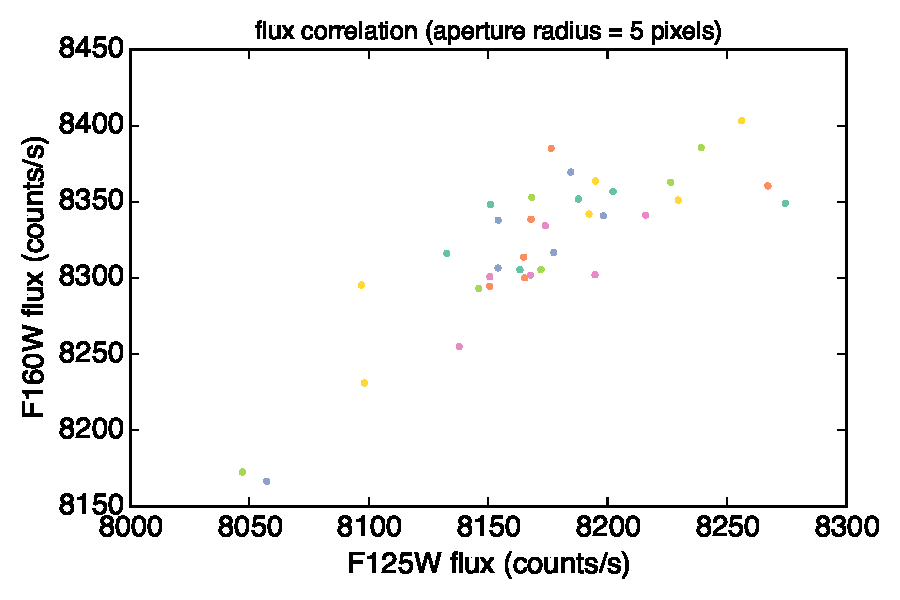
\includegraphics[width=0.8\textwidth]{Flux_correlation_Nov17}
  \caption{F160W flux vs. F125W flux. Different colors indicate
    different orbits.}
  \label{fig:corr}
\end{figure}

\begin{quote}
  color magnitude diagram (Apai 2013)
\end{quote}
I was confused about magnitude system when converting fluxes to
magnitudes. STSCI provides three magnitude systems, ST magnitude, AB
magnitude, and vega magnitude. I used both AB magnitude and vega
magnitude for conversion and listed the plots in figure \ref{fig:cmd}.

\begin{figure}
  \centering
  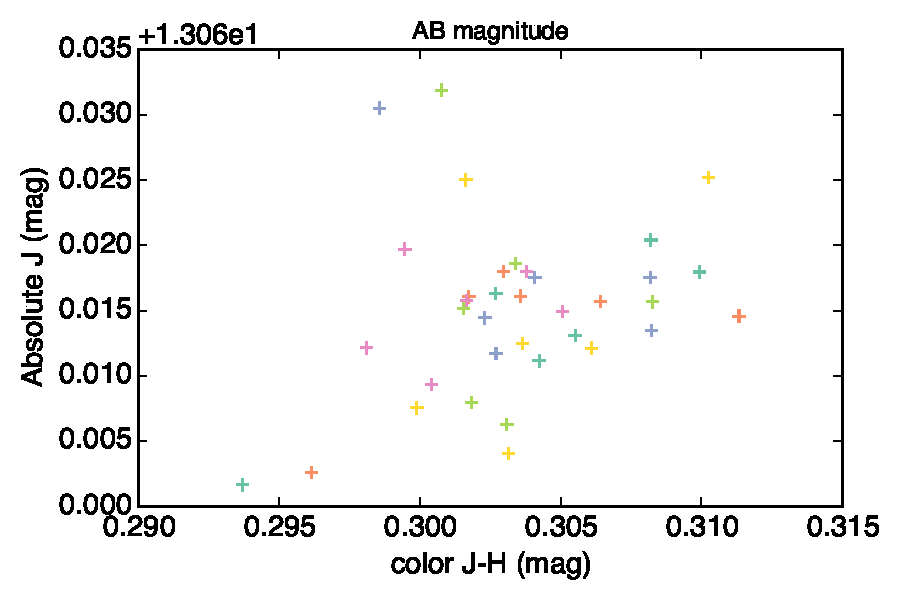
\includegraphics[width=0.8\textwidth]{CMD_ABmag_Nov20}
  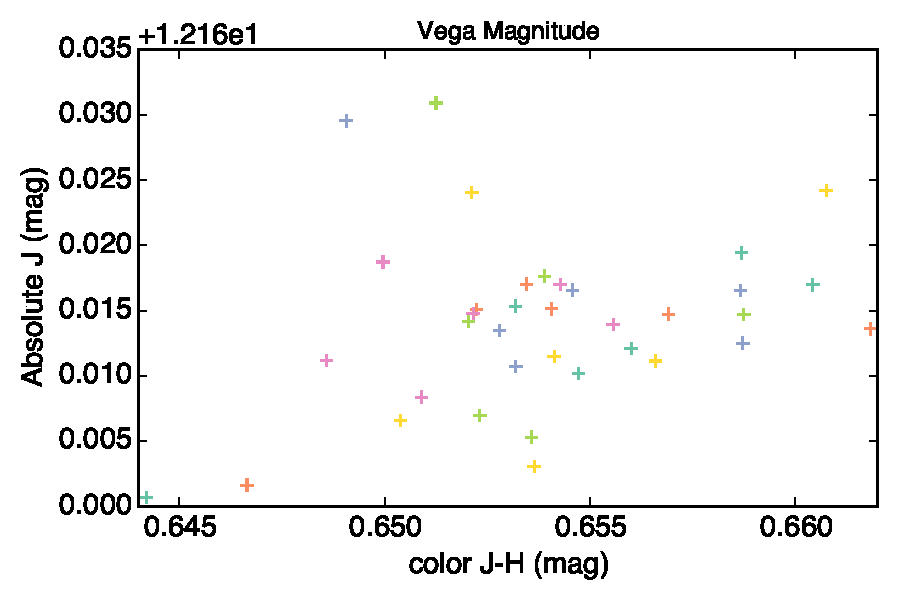
\includegraphics[width=0.8\textwidth]{CMD_Vegamag_Nov20}
  \caption{color magnitude diagram, different colors indicate
    different orbits}
  \label{fig:cmd}
\end{figure}


\section{Optimization of Aperture Size}

Optimum aperture size is related to the estimation of background
fluctuation. A difference of 1 count/pixel difference in background
fluctuation could lead to 0.5 pixel change in optimum aperture
radius. Aper.pro routine provides 2 ways to define sky fluctuation:
\begin{enumerate}
\item directly input sky level and fluctuation when calling the program. The sky value and sigma should be calculated before hand.
\item  input annulus radii of the sky region and let the program calculate it. The sky region here must be an annulus around the secondary object in this case.
\end{enumerate}
I choose to calculate the sky fluctuation separately rather than let aper.pro calculate.     

\begin{enumerate}
\item if the annulus is too close to the secondary object, the flux of the secondary image could contaminate the sky and end up with a higher estimation of sky level and an inaccurate estimate of sky fluctuation.    
\item The annulus radii cannot be large too. Because the slight change of
PSF, the image of the primary cannot be removed completely. The
residual of the primary image fluctuate largest at the center region
as well as the diffraction spikes region.  When the annulus radii get
slightly larger, the annulus would include these region. If the
annulus radii get even larger to avoid these region, it would cause an
under-estimate of the sky fluctuation because the area of this annulus
is not affected by psf subtraction.
\end{enumerate}

The optimum aperture radius turned out to be very small, it ranges from 2.8 to 3.5 pixels. which is only 1 pixel larger than fwhm of the image, which is 1.8 pixels.
\end{document}

%%% Local Variables:
%%% mode: latex
%%% TeX-master: t
%%% End:
